\documentclass[a4paper, 12pt]{article}

%Абзацный отступ

\usepackage{indentfirst}

%Рисунки

\usepackage{subfig}
\usepackage{graphicx}
\usepackage{wrapfig}

%Гиперссылки и работа с цветом

\usepackage{hyperref}
\usepackage[rgb]{xcolor}
\hypersetup{			%Гиперссылки
	colorlinks=true, 	%false: ссылки в рамках
	urlcolor=blue		%на URL
}

%Русский язык

\usepackage[T2A]{fontenc}		%кодировка
\usepackage[utf8]{inputenc}		%кодировка исходного текста
\usepackage[english, russian]{babel}	%локализация и переносы


%Математика

\usepackage{amsmath, amsfonts, amssymb, amsthm, mathtools, mathrsfs}

%Пакет с градусом

\usepackage{gensymb}


\author{Штрайх Роберт}
\title{Работа 4.3.3. Исследование разрешающей способности микроскопа методом Аббе}
\date{09 февраля 2022 г.}

\begin{document}
\begin{titlepage}
	\centering
	\vspace{5cm}
	{\scshape\LARGE Московский физико-технический институт \par}
	\vspace{4cm}
	{\scshape\Large Лабораторная работа №4.4.1 \par}
	\vspace{1cm}
	{\huge\bfseries Амплитудная дифракционная решётка\par}
	\vspace{1cm}
	\vfill
\begin{flushright}
	{\Large выполнили студенты 006 и 007 группы ФЭФМ}\par
	\vspace{0.3cm}
	{\Large Штрайх Роберт}\par
	\vspace{0.3cm}
	{\Large Петрова Софья}
\end{flushright}
	

	\vfill

% Bottom of the page
	Долгопрудный, 2022 г.
\end{titlepage}

\newpage

\textbf{Цель работы:} Знакомство с работой и настройкой гониометра Г5, определение спектральных характеристик амплитудной решетки.

\textbf{В работе используются:} гониометр, дифракционная решетка, ртутная лампа.

\section*{Теоретическое введение}

\noindent 1. Основное соотношение приближенной теории дифракционной решётки:
	\begin{equation}
	d\sin \varphi_m = m\lambda.
	\end{equation}
	Угловая дисперсия $D$ характеризует угловое расстояние между близкими спектральными линиями:
	\begin{equation}
	D = \frac{d\varphi}{d\lambda} = \frac{m}{d \cos \varphi}=\frac{m}{\sqrt{d^{2}-m^{2} \lambda^{2}}}.
	\end{equation}
Т.е. это производная зависимости угла отклонения волны диспергирующим элементом по длине волны.

\noindent 2. Разрешающая способность $R = \dfrac{\lambda}{\delta \lambda}$ характеризует возможность прибора различать две близкие спектральные линии с длинами волн $\lambda$ и $\lambda + \delta \lambda$.

\noindent 3. Также стоит выделить дисперсионную область, которая является предельной шириной спектрального интервала $\Delta \lambda$ прибора, для которой дифракционные максимумы соседних порядков не перекрываются. Она определяет диапазон длин волн, при которых прибор может быть использован для анализа спектра.
Полуширина линии $\delta \varphi = \dfrac{\lambda}{Nd\cos \varphi}$.
Разрешающую способность в силу критерия Релея можно записать в следующем виде $R = Nm$.

\begin{figure}[h]
\begin{center}
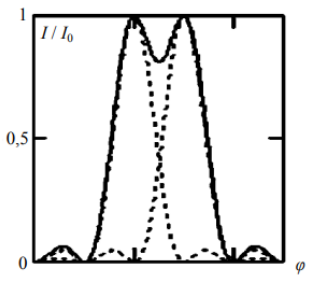
\includegraphics[width=0.3\textwidth]{Критерий_Релея.png}
\end{center}
\caption{Иллюстрация к критерию Релея} \label{Критерий Релея}
\end{figure}

\section*{Экспериментальная установка}

\subsection*{Устройство гониометра Г5}

\begin{figure}[h]
\begin{center}
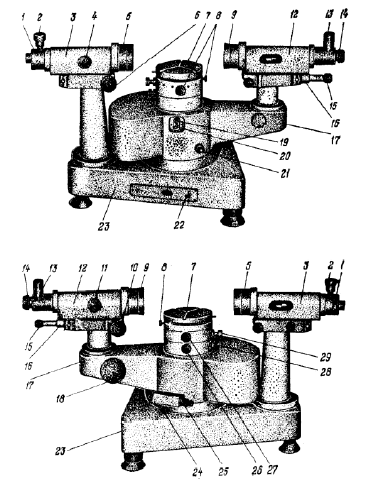
\includegraphics[width=0.8\textwidth]{Гониометр.png}
\end{center}
\caption{Гониометр Г5} \label{Гониометр}
\end{figure}

Опишем некоторые обозначенные на рисунке гониометра элементы. Коллиматор 3, столик 7 и алидада 17 со зрительной трубе 12 крепится на массивном основании 23. На столике 7 размещаются исследуемые объекты. Коллиматор закреплен неподвижно, а столик и алидада с трубой могут вращаться вокруг вертикальной оси.

\subsection*{Дифракционная решетка}

При работе с дифракционной решеткой основной задачей является точное измерение углов, при которых наблюдаются главные максимумы для различных длин волн. В нашей работе для измерения углов используется гониометр Г5. 

\begin{figure}[h]
\begin{center}
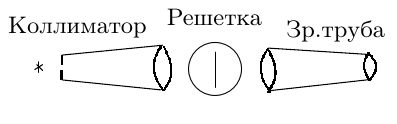
\includegraphics[width=0.6\textwidth]{Принципиальная_схема_установки.png}
\end{center}
\caption{Принципиальная схема установки} \label{Схема}
\end{figure}

\subsection*{Спектр ртутной лампы}

Каждая линия спектра имеет свою ширину и тонкую структуру. Ниже приведены некоторые интегральные характеристики спектральных линий для лампы ДРШ - 250.

\begin{figure}[h]
\begin{center}
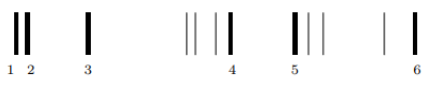
\includegraphics[width=0.6\textwidth]{Спектр.png}
\end{center}
\caption{Спектр ртутной лампы ДРШ-250} \label{Спектр}
\end{figure}

\begin{figure}[h]
\begin{center}
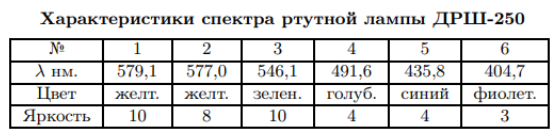
\includegraphics[width=0.8\textwidth]{Характеристики.png}
\end{center}
\caption{Характеристики ДРШ-250} \label{Характеристики ДРШ}
\end{figure}

\section*{Ход работы}

\noindent 1. Измерим угловые координаты спектральных линий ртути в $\pm 1$ порядках ($\sigma_\varphi = 2.4 \cdot 10^{-5}$ рад).

\begin{table}[h!]
\centering
\label{Углы}
\begin{tabular}{|l|l|l|l|l|l|l|l|}
\hline
Цвет        & фиолетовый & голубой & зеленый & желтый & желтый & красный & красный \\ \hline
$\varphi$        & 11,77      & 13,7    & 15,7    & 16,75  & 16,79  & 17,63   & 17,78   \\ \hline
$\sin \varphi$       & 0,204      & 0,237   & 0,271   & 0,288  & 0,289  & 0,303   & 0,305   \\ \hline
$\lambda$, нм & 404,66     & 491,6   & 546,07  & 576,96 & 579,07 & 623,4   & 690,72  \\ \hline
\end{tabular}
\caption{Результаты измерений угловых координат спектральных линий}
\end{table}

\begin{figure}[h!]
\begin{center}
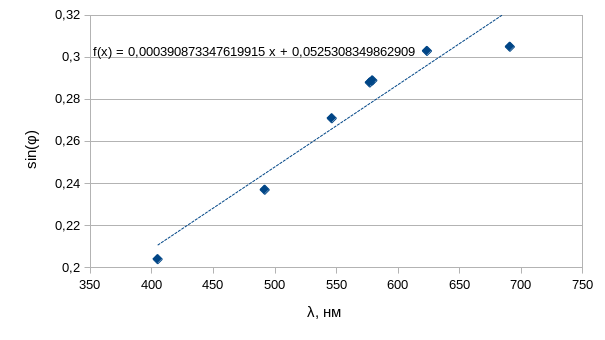
\includegraphics[width=1\textwidth]{graph1.png}
\end{center}
\caption{Зависимость $\sin \varphi (\lambda)$} \label{Лямбда от фи}
\end{figure}

Определим период решетки:

\[\sigma_d = \sigma_{\dfrac{1}{k}} =\dfrac{1}{\sqrt{n}}\sqrt{\dfrac{<\lambda \sin \varphi> - <\lambda> <\sin \varphi>}{<\sin^2 \varphi> - <\sin \varphi>^2}}\]

\[d = \dfrac{1}{k} = (2558 \pm 250) \text{ нм}\]

\noindent 2. Рассчитаем и сравним между собой экспериментальную и теоретическую угловую дисперсию для желтого дублета в спектрах разного порядка. Для расчета теоретической дисперсии возьмем среднюю длину волны желтого дублета.

\[D_\text{т} = \dfrac{m}{\sqrt{d^2-m^2 \lambda^2}} \text{;}~~ \sigma_{D_\text{т}} = \dfrac{md}{(d^2-m^2 \lambda^2)^{3/2}}\]

\begin{table}[h!]
\centering
\label{Теор дисперсия}
\begin{tabular}{|l|l|l|l|}
\hline
$m$     & 1                           & 2             & 3\\ \hline
$D_\text{т} \cdot 10^{-5}$, рад/$\text{\AA}$   & 4,01 & 8,76  & 15,93   \\ \hline
$\sigma_{D_\text{т}} \cdot 10^{-9}$, рад/$\text{\AA}$ & 1,65 & 4,3 & 11,49\\ \hline
\end{tabular}
\caption{Теоретически рассчитанная угловая дисперсия}
\end{table}
 
Для оценки экспериментальной угловой дисперсии определим разности угловых координат линий желтого дублета во всех видимых порядках ($\Delta \lambda = 21 \text{ \AA}$): 

\[D_\text{э} = \dfrac{\Delta \varphi}{\Delta \lambda}\]

\[\sigma_{\Delta \varphi} = \sqrt{2} \sigma_\varphi = 3.39 \cdot 10^{-5}~\text{рад}\]

\[\dfrac{\sigma_{D_\text{э}}}{D_\text{э}}=\dfrac{\sigma_{\Delta \varphi}}{\Delta \varphi}\]

\begin{table}[h!]
\centering
\label{Эксперимент дисперсия}
\begin{tabular}{|l|l|l|l|}
\hline
$m$                                & 1     & 2   & 3   \\ \hline
$D_\text{э} \cdot 10^{-5}$, рад/$\text{\AA}$ & 3,02  & 8,04  & 17,01 \\ \hline
$\sigma_{D_\text{э}} \cdot 10^{-6}$, рад/$\text{\AA}$ & 1,61 & 1,61 & 1,62\\ \hline
$\Delta \varphi \cdot 10^{-5}$, рад                        & 63,42 & 168,84 & 357,21\\ \hline
\end{tabular}
\caption{Экспериментально найденная угловая дисперсия}
\end{table}

Значения угловой дисперсии с повышением порядка спектра линейно возрастают.

\clearpage
\begin{figure}[h!]
\begin{center}
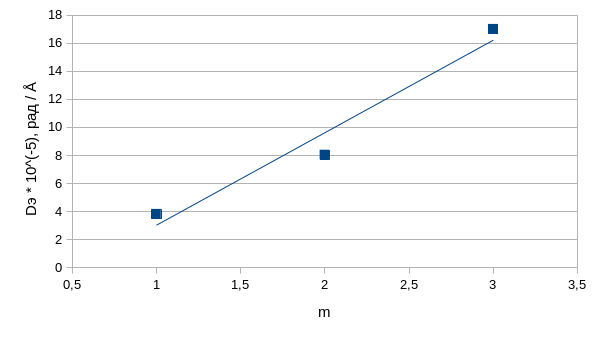
\includegraphics[width=0.8\textwidth]{graph2.png}
\end{center}
\caption{Зависимость $D_\text{э}(m)$} \label{D от фи}
\end{figure}

\noindent 3. Оценим разрешимый спектральный интервал $\delta \lambda$, зная угловую полуширину желтой линии и угловую дисперсию. Ширина одной из линий желтого дублета 47'' = $2.277 \cdot 10^{-4}$ рад:

\[\dfrac{\sigma_{\delta \lambda}}{\delta \lambda} = \sqrt{\left(\dfrac{\sigma_{\Delta \varphi}}{\Delta \varphi}\right)^2 + \left(\dfrac{\sigma_D}{D}\right)^2}\]

\[\delta \lambda \approx \dfrac{\Delta \varphi}{D} = (2.8 \pm 0.49) \text{ \AA}\]

Оценим разрешающую способность для средней длины волны жёлтого дублета:

\[\dfrac{\sigma_R}{R} = \dfrac{\sigma_{\delta\lambda}}{\delta \lambda}\]

\[R = \dfrac{\lambda}{\delta \lambda} = (2060.71 \pm 360.62)\] 

Оценим число эффективно работающих штрихов решётки и её эффективный размер:

\[\dfrac{\sigma_N}{N} = \dfrac{\sigma_R}{R}\]

\[N = \dfrac{R}{m} = (1030 \pm 180)\]

\[\dfrac{\sigma_l}{l} = \sqrt{\left(\dfrac{\sigma_N}{N}\right)^2 + \left(\dfrac{\sigma_d}{d}\right)^2}\]

\[l = Nd \approx (2.63 \pm 0.52) \text{ мм}\]

\noindent 4. Рассчитаем порядок спектра, при котором фиолетовая линия наложится на желтую:

\[m = \dfrac{\lambda}{\Delta \lambda} \approx 192\]

\section*{Выводы}

\begin{itemize}
\item Мы ознакомились с устройством и работой гониометра, произвели его юстировку.

\item Определили спектральные характеристики используемой в работе амплитудной решетки: её шаг, угловую дисперсию, число эффективно работающих штрихов и эффективный размер решётки.
\end{itemize}
 
\end{document}